\documentclass{article}
\usepackage[letterpaper, margin = 1in]{geometry}
\usepackage[usenames, dvipsnames]{color}
\usepackage{graphicx}
\usepackage{amsmath, amssymb}
\usepackage{amsfonts}
\usepackage{cancel}
\usepackage{soul}

\begin{document}

\title{CS229 : Project Milestone}
\author{Jee Ian Tam (jeetam), Sean Rafferty (seanraff)}

\section{Introduction}
There are a large number of open live webcams that are accessible over the internet. Such webcams can show interesting content from various places all around the world, but it is not feasible for a single person to browse all of the webcams to search for such interesting content. Our project aims to use Machine Learning algorithms to cluster and identify webcams of interest out of a large pool of webcams. \\

We scrape a list of publicly accessible, non-password-protected webcams from opentopia.com. The website provides metadata about the webcam (GPS coordinates, location name, local time) as well as a URL which can be used to retreive a snapshot of the most recent image for a webcam. We log images from 2000 webcams with a 5-minute recording period over a duration of 1 week. The goal is to train our Machine Learning algorithms on this training data set, and then test them on the live webcams. \\

A large majority of webcams at any one time do not display anything interesting, and simply show a static background. An interest metric that we can define is a measure of the activity that is occurring as recorded by the webcam. In order to highlight webcams that have a high interest metric, we use a background subtraction algorithm combined with some post-processing to detect foregound objects against the background recorded by the webcam. This is detailed in section 2. \\

Another method that we use to explore the data set is to perform K-means clustering on the webcam images to see if the webcams in the data set can be meaningfully clustered. For example, in the data set there could be a cluster of webcams that are located outdoors, a cluster of webcams that show natural scenery, a cluster of webcams that show images of towns around the world, etc. \textcolor{red}{[! Sean to add more stuff here about context/results behind K-means!]} \\ 

\section{K-means}

\section{Background Subtraction and Activity Detection}
In order to calculate the interest metric of a webcam, the first step is to perform background subtraction on the stream of images coming from a webcam. The goal of this is to effectively detect activity from foreground objects (for example cars, people, animals, etc.), and to do this it is necessary to train a classifier to classify foreground objects from the background. \\

To classifiy foreground objects from the background view of a webcam, we train each pixel on a Gaussian Mixture Model (GMM) in an unsupervised learning approach. Each pixel is treated as a vector in the $\mathbb{R}^3$ RGB space, and is given as input to the GMM to be trained in an online learning method. The number of Gaussians is adjusted adaptively. We use the BackgroundSubtractorMOG2() function in the Python OpenCV library to perform this background subtraction algorithm. The function implements the background subtraction algorithm as detailed by Z. Zivkovic \footnote{Z.Zivkovic, Improved adaptive Gausian mixture model for background subtraction, International Conference Pattern Recognition, UK, August, 2004, http://www.zoranz.net/Publications/zivkovic2004ICPR.pdf.}.\\

Initial testing of the interest metric as a function of the number of classified foreground pixels revealed a flaw in this naive approach : The foreground detection algorithm suffers from abrupt lighting changes, which happen very often due to many webcams adjust their aperture dynamically in response to local lighting conditions. Such occurrences cause the classifier to erroneously classify a large number of background pixels as foreground. Thus, this interest metric results in the algorithm giving many false positives, returning images that had a change in lighting conditions without any noticeable change in the background or foreground. Thus, this initial approach did not yield acceptable results. See Figure \ref{Fig:LightingConditions} for an example. \\

In order to handle the false positives from this naive implementation, we introduce an additional post-processing step to reduce the effect of lighting conditions on the interest metric. Since the foreground detection algorithm returns a mask where background pixels are colored black and foreground pixels are colored white, foreground objects show up as white "blobs" against the black background of the mask. The main observation (or assumption) is that the blobs of objects of interest (e.g. cars, people, animals, etc.) are small relative to the size of the image. Thus, if we can base our interest metric on some function of the blobs and threshold the blobs based on their size, we can improve the background subtraction pipeline's ability to handle changes in lighting condition. \\

We use the SimpleBlobDetector() function in the Python OpenCV library to fit contours around each blob, and threshold each blob based on a maximum percentage (nominally 20\%) of the total image area. Furthermore, we now define the interest metric to be a function of the total area of blobs that occupy an image foreground. This has the effect of assigning more weight to foreground objects that are more prominent (have larger area) in the webcam image, which is what is desired. Adding this post-processing step and redefining the interest metric to be a function of the total area of blobs results in an improved webcam highlighting algorithm that is more robust to lighting changes in webcams. See Figure \ref{Fig:ForegroundDetection} for an example. \\

Even though we have made the webcam highlighting more robust against lighting changes, it is still not robust against webcams that move around, causing the background to shift constantly. The resulting background model from the background subtraction algorithm is not representative of the actual background that the webcam is pointing at, resulting in poor object detection performance. One possible way to address this would be to use the blob detection post-processing step above to check if a large portion of the image has changed, and block or refresh the background model to take into account that the background has changed.\\

Another improvement that can be made to the interest metric is to take into include the element of time into the calculation. Currently the webcams are highlighted based on the current webcam image that has the highest foreground blob areas, without consideration for the past history of the webcams. However, one possible way to improve the performance of the webcam highlighting might be to factor in the frequency and/or duration of the observed activity - That is, highlight a webcam only when we observe sustained activity over a pre-defined duration of time. 

\section{Further work}

\newpage

\section{Appendix}
\begin{figure}[h]
\centering
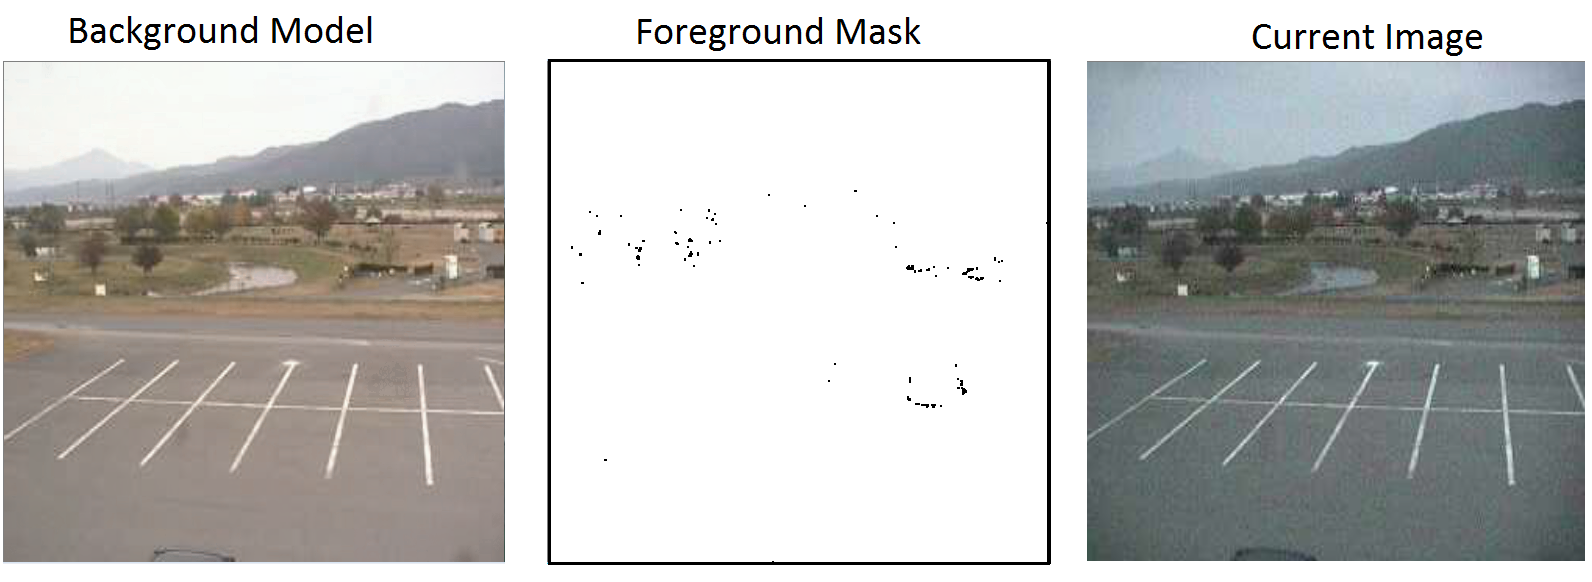
\includegraphics[scale = 0.4]{LightingConditions}
\caption{Failure of Naive background subtraction model to handle lighting changes}
\label{Fig:LightingConditions}
\end{figure}
\begin{figure}[h]
\centering
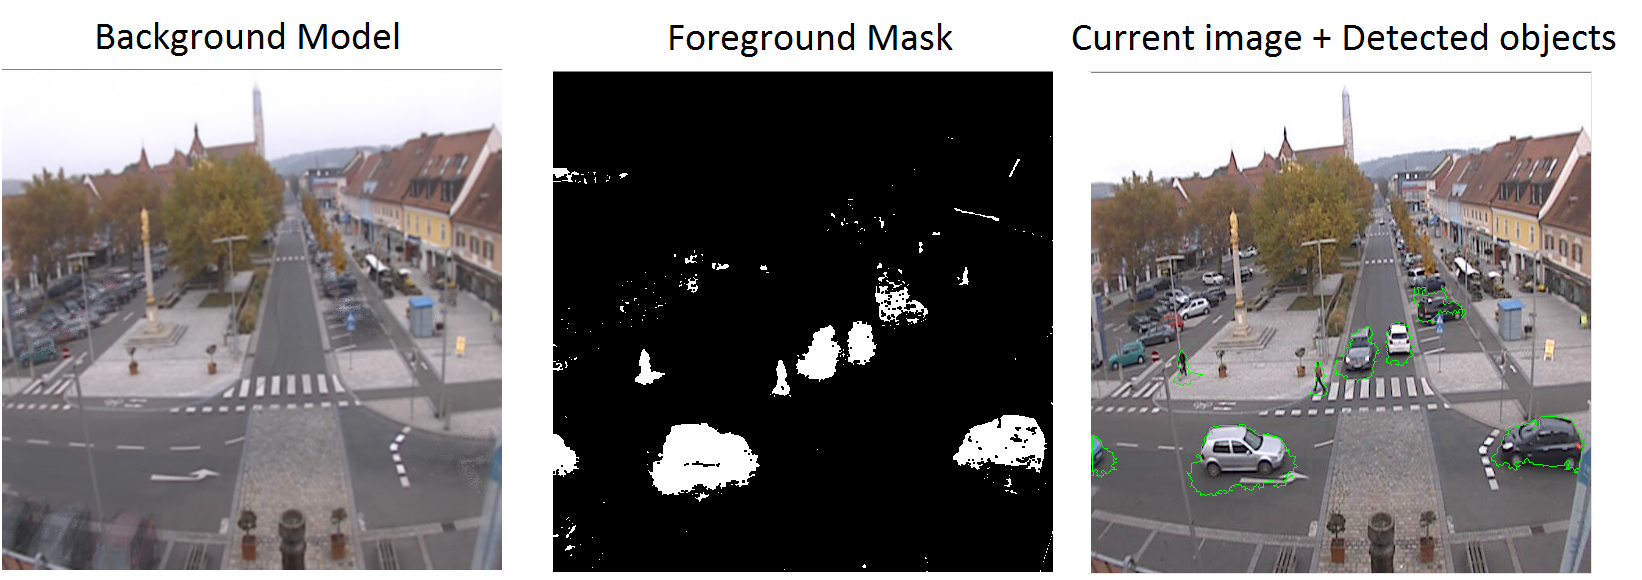
\includegraphics[scale = 0.4]{BackgroundSubtraction1}
\caption{Example of background/foreground segmentation algorithm}
\label{Fig:ForegroundDetection}
\end{figure}






\end{document}